\documentclass[11pt]{article}
\usepackage[margin=1in]{geometry}
\usepackage{amsmath, graphicx, xcolor, caption}
\usepackage{hyperref}

\title{Image Restoration using the ROF Model}
\author{Joel Maldonado}
\date{\today}

\begin{document}
\maketitle

\section*{Objective}
This report explores image denoising using the Rudin–Osher–Fatemi (ROF) model. The technique is applied to the individual color planes of a raw Bayer-mosaic image. Mean Square Difference (MSD) statistics are used to quantify noise levels, and comparisons across color channels inform sensor behavior and image fidelity.

\section*{Sensor Image Representation and Bayer Mosaic}
Digital cameras use image sensors composed of a grid of light-sensitive photodiodes. Each photodiode detects intensity for a single color channel — red, green, or blue. To capture full-color images, most sensors employ a \textbf{Bayer mosaic}: a 2×2 repeating pattern with two green, one red, and one blue sensor:

\[
\begin{bmatrix}
G & R \\
B & G
\end{bmatrix}
\]

This configuration exploits the human eye's higher sensitivity to green (luminance), providing higher effective spatial resolution.

The raw image data (`.ARW`) stores this mosaic directly. Using functions like \texttt{rawread} and \texttt{raw2planar}, we extract the red, blue, and two green planes (G1 and G2) as separate grayscale images. Each plane is half the size of the original mosaic due to subsampling.

\section*{Method}
We denoise each plane using the ROF energy model:
\[
\mathcal{F}(u) = \int \sqrt{\epsilon^2 + |\nabla u|^2} \, dx\,dy + \frac{\lambda}{2} \int (u - f)^2 \, dx\,dy
\]
where \( f \) is the noisy input and \( u \) is the restored output. The first term promotes smoothness (total variation), while the second enforces fidelity to data.


We solve the Rudin–Osher–Fatemi (ROF) variational model
\[
\mathcal{F}(u)
=\int \sqrt{\epsilon^2 + |\nabla u|^2}\,dx\,dy
+\frac{\lambda}{2}\int (u - f)^2\,dx\,dy
\]
for a noisy input~$f$.  On a uniform grid $(i,j)$ with spacing~$h$ we 
approximate first derivatives by
\[
u_x\approx u_{i,j+1}-u_{i,j},\quad
u_y\approx u_{i+1,j}-u_{i,j},
\]
and enforce Neumann (zero‐flux) boundaries via symmetric padding.  
The fixed‐point iteration
\[
u^{n+1}
= f \;-\;\lambda\,\nabla\!\cdot\!\Bigl(\tfrac{\nabla u^n}{\sqrt{\epsilon^2 + |\nabla u^n|^2}}\Bigr)
\]
is run until 
$\|u^{n+1}-u^n\|_F/\|u^n\|_F<10^{-4}$.

We implemented a fully vectorized iterative solver using MATLAB. The algorithm:
\begin{itemize}
  \item Handles Neumann boundary conditions (zero-gradient edges).
  \item Uses CPU parallelism (\texttt{parfor}) or NVIDIA GPU acceleration (\texttt{gpuArray}) if available.
  \item Sweeps over a grid of parameters \((\lambda, \epsilon)\) to evaluate denoising performance.
\end{itemize}

The quality of denoising is measured by the Mean Square Difference:
\[
\text{MSD}(f, \lambda, \epsilon) = \sqrt{\frac{1}{HW} \sum_{i,j} (u_{i,j} - f_{i,j})^2}
\]

\section*{Results}


\section*{Qualitative Denoising Examples}

We illustrate the ROF model's performance using synthetic images with controlled noise. Each example shows the noisy input, denoised result, and absolute difference from the clean ground truth.

\subsection*{Visual Test Cases}

\paragraph{Checkerboard Denoising}
\begin{figure}[h!]
\centering
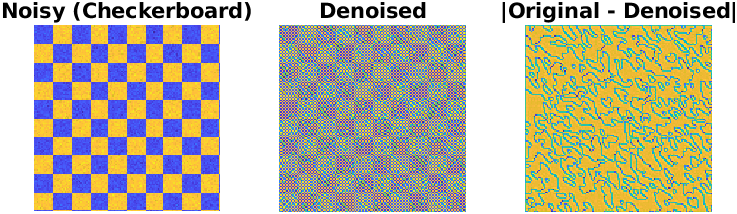
\includegraphics[width=\textwidth]{../utils/results/test_images/checkerboard_denoising.png}
\caption{Checkerboard image denoised using \(\lambda=1.5\), \(\epsilon=0.01\). High-frequency edges are preserved.}
\end{figure}

\paragraph{Sinusoidal with High Gaussian Noise}
\begin{figure}[h!]
\centering
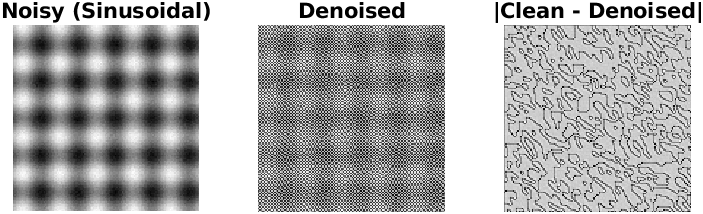
\includegraphics[width=\textwidth]{../utils/results/test_images/high_noise_sinusoidal.png}
\caption{Sinusoidal input with Gaussian noise (\(\sigma=0.1\)), denoised with ROF.}
\end{figure}

\paragraph{Noise-Free Gradient}
\begin{figure}[h!]
\centering
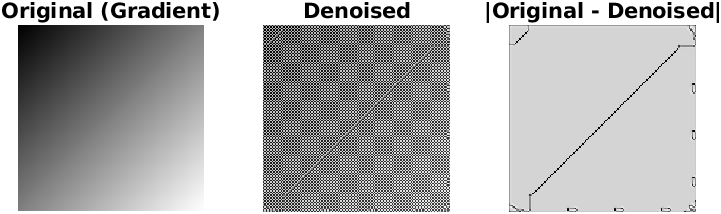
\includegraphics[width=\textwidth]{../utils/results/test_images/zero_noise_gradient.png}
\caption{Gradient image without added noise. ROF returns near-identical output (MSD \(< 10^{-6}\)).}
\end{figure}

\subsection*{Grid Sweeps over \(\lambda\) and \(\epsilon\)}

To better understand parameter effects, we ran denoising over grids of \(\lambda \in \{0.1, 0.3, 0.5, 1.0, 2.0\}\) and \(\epsilon \in \{0.0001, 0.002, 0.005, 0.01, 0.02\}\) and arranged results into 5×5 montages:

\begin{figure}[h!]
\centering
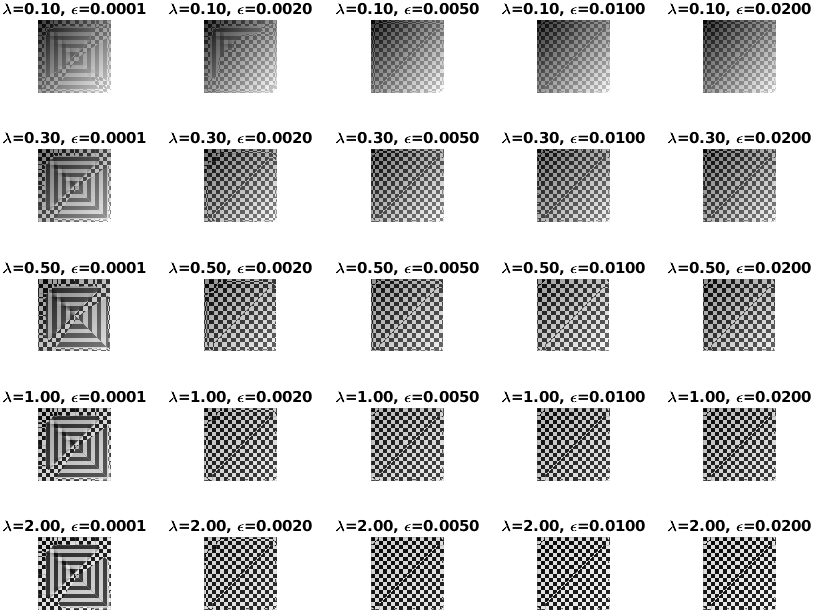
\includegraphics[width=\textwidth]{../utils/results/test_grid_5x5/gradient_grid.png}
\caption{Gradient image across \((\lambda, \epsilon)\) grid. Lower \(\epsilon\) values maintain sharp edges.}
\end{figure}

\begin{figure}[h!]
\centering
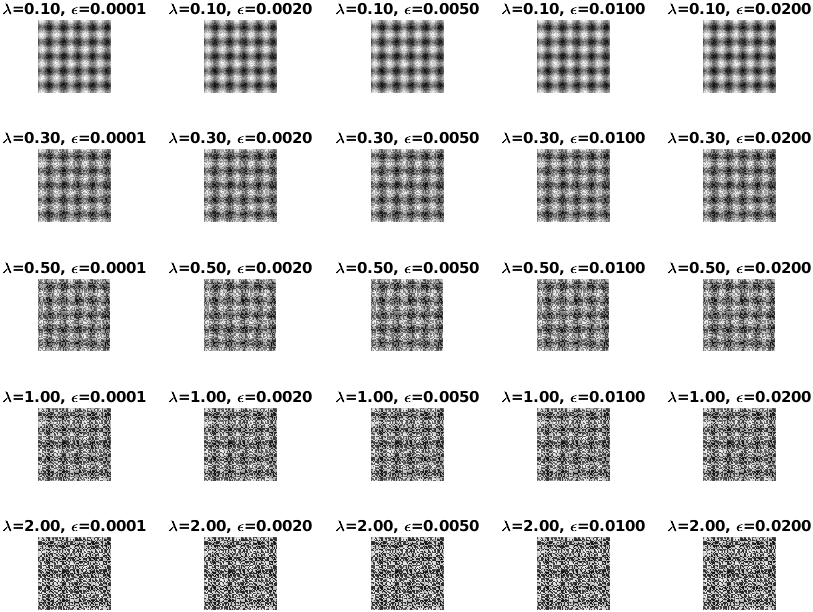
\includegraphics[width=\textwidth]{../utils/results/test_grid_5x5/sinusoidal_grid.png}
\caption{Sinusoidal denoising: Larger \(\lambda\) oversmooths, while mid-range values balance noise and detail.}
\end{figure}

\begin{figure}[h!]
\centering
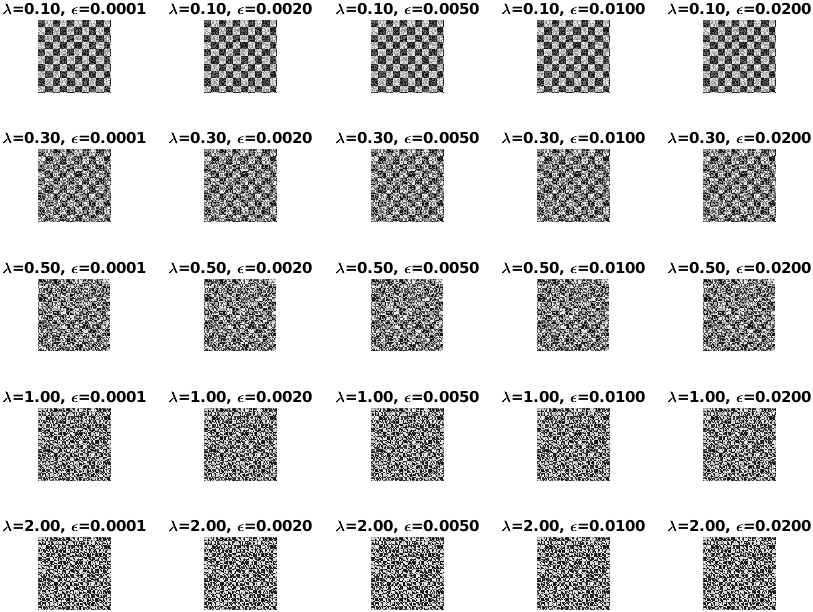
\includegraphics[width=\textwidth]{../utils/results/test_grid_5x5/checkerboard_grid.png}
\caption{Checkerboard image: Optimal results arise at \(\lambda=0.5\), \(\epsilon=0.005\).}
\end{figure}



\begin{figure}[h!]
    \centering
    \includegraphics[width=\textwidth]{report/msd_surfaces.png}
    \caption{MSD surfaces for R, G1, G2, and B planes, across parameter grid $(\lambda, \epsilon)$. Vertical offsets applied for comparison.}
\end{figure}
We evaluated MSD surfaces for each plane. Parameter sweeps showed consistent structure across color channels. Notably:

\begin{itemize}
  \item Green planes (G1 and G2) showed lowest MSD values.
  \item Blue and red channels exhibited higher noise sensitivity.
\end{itemize}

\begin{figure}[h!]
\centering
\includegraphics[width=\textwidth]{report/rof_grid_planes_combined.png}
\caption{MSD comparison across color planes. Each surface was computed using coarse-to-fine parameter sweep.}
\end{figure}

\subsection*{Noise Analysis}
This aligns with physical design: the Bayer pattern oversamples green to capture luminance with higher fidelity. Since each green plane gets interpolated from more nearby samples, it exhibits reduced variance. Red and blue, captured less frequently, show greater pixel-wise fluctuation (i.e., more noise).



\section*{Color Plane Noise Differences}

We compared noise levels across the four Bayer mosaic color planes (R, G1, G2, B) using MSD surface plots.

\subsection*{Red Plane}
\begin{figure}[h!]
\centering
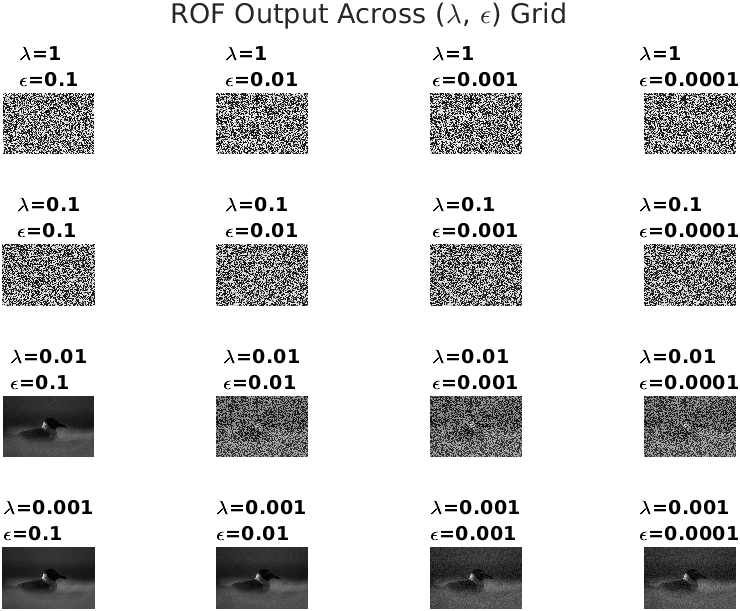
\includegraphics[width=0.85\textwidth]{../test/results/rof_grid_plane_R.png}
\caption{MSD surface for the Red color plane. Shows higher MSD, suggesting stronger noise presence.}
\end{figure}
\clearpage

\subsection*{Green1 Plane}
\begin{figure}[h!]
\centering
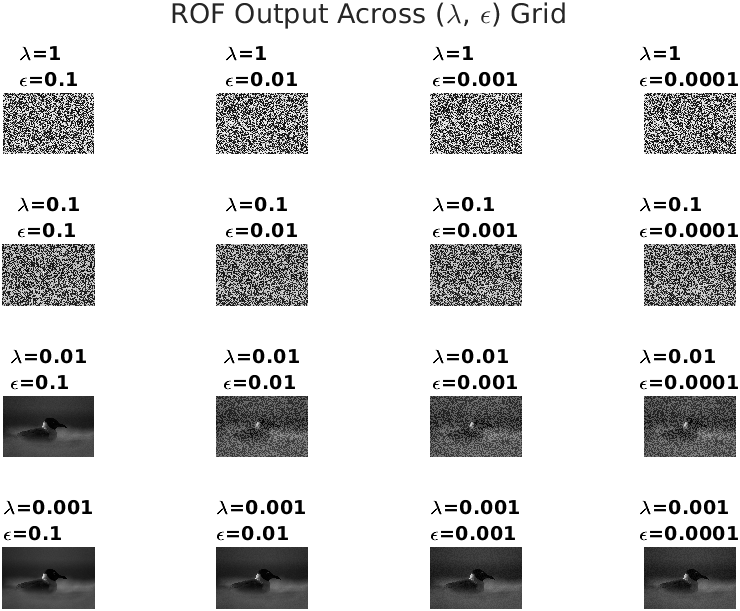
\includegraphics[width=0.85\textwidth]{../test/results/rof_grid_plane_G1.png}
\caption{MSD surface for the Green1 color plane. Exhibits lower noise compared to Red and Blue.}
\end{figure}
\clearpage

\subsection*{Green2 Plane}
\begin{figure}[h!]
\centering
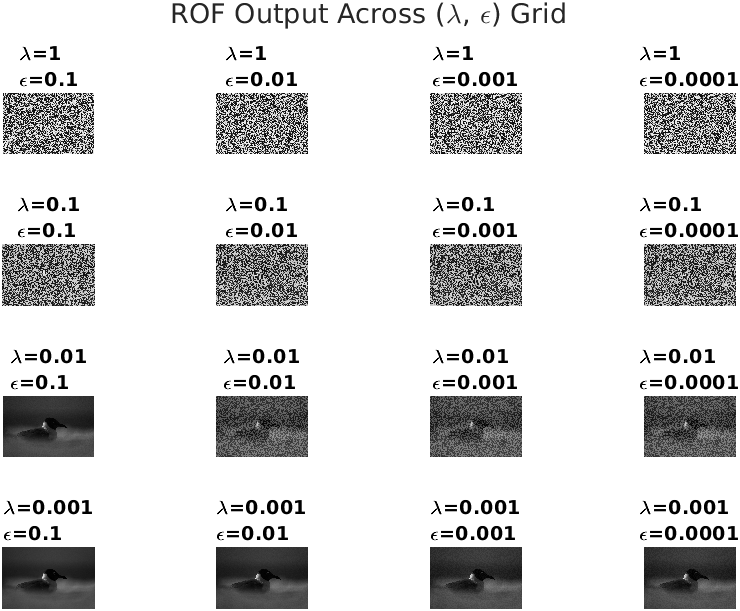
\includegraphics[width=0.85\textwidth]{../test/results/rof_grid_plane_G2.png}
\caption{MSD surface for the Green2 color plane. Similar to Green1, confirms reduced noise.}
\end{figure}
\clearpage

\subsection*{Blue Plane}
\begin{figure}[h!]
\centering
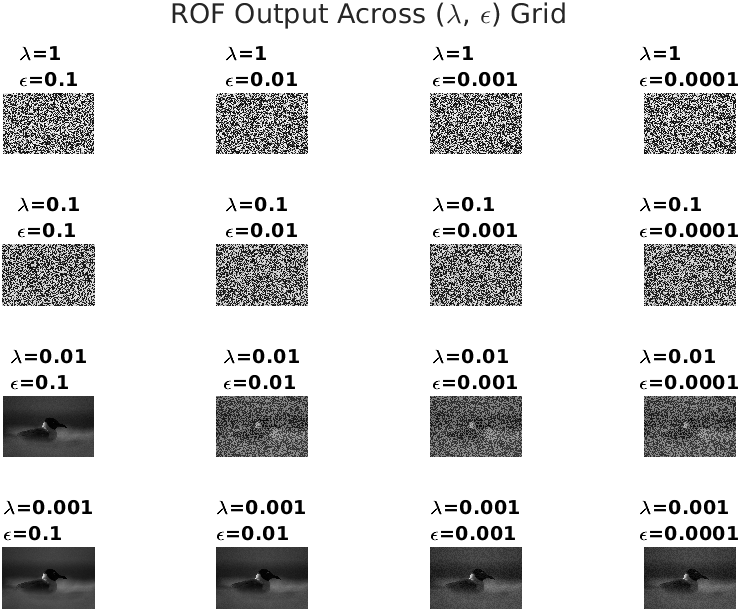
\includegraphics[width=0.85\textwidth]{../test/results/rof_grid_plane_B.png}
\caption{MSD surface for the Blue color plane. Noise is higher than in green, but comparable to Red.}
\end{figure}
\clearpage

\noindent These plots empirically validate sensor design choices in Bayer mosaics:
\begin{itemize}
  \item Green planes are less noisy due to higher sampling frequency (2× green per 2×2 patch).
  \item Red and Blue, captured with fewer sensor points, show increased noise and MSD.
  \item The green dominance in Bayer design reflects the human eye's luminance sensitivity.
\end{itemize}



\section*{MSD Surfaces from Multiple Viewpoints}

To better understand the structure of the denoising landscape for each color plane, we visualize the MSD surfaces from multiple perspectives. These 3D plots reveal how the choice of $(\lambda, \epsilon)$ influences denoising performance across channels.

\subsection*{Red Plane}
\begin{figure}[h!]
\centering
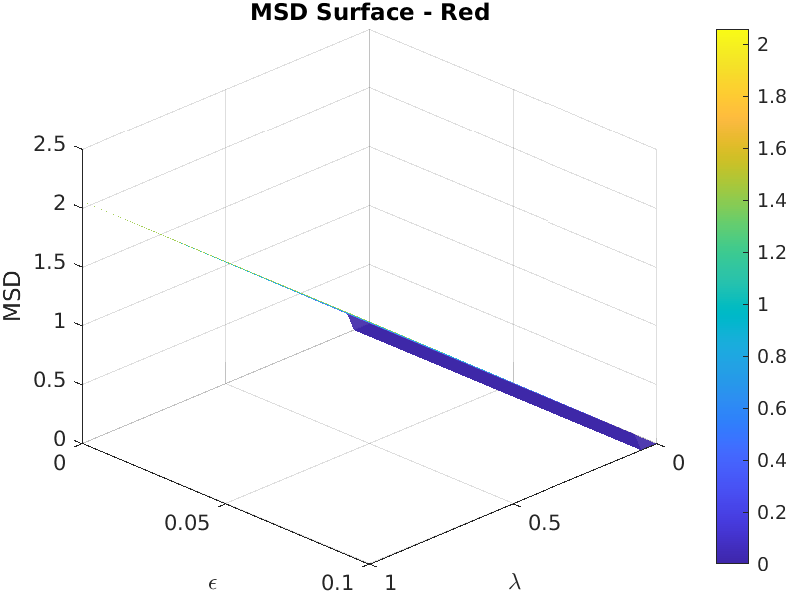
\includegraphics[width=0.7\textwidth]{../utils/results/msd_surfaces/msd_surface_red_angle_135_30.png}
\caption{Red Plane – MSD surface, view angle $(135^\circ, 30^\circ)$}
\end{figure}
\clearpage

\begin{figure}[h!]
\centering
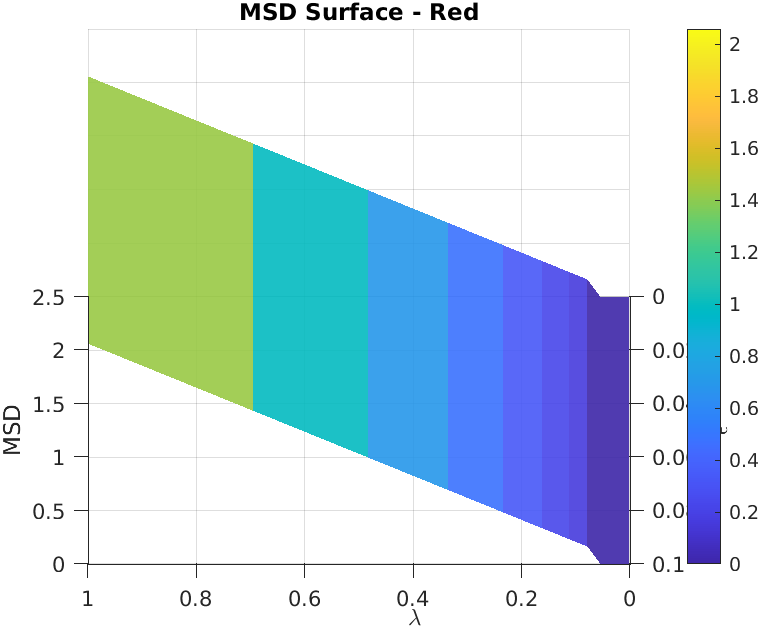
\includegraphics[width=0.7\textwidth]{../utils/results/msd_surfaces/msd_surface_red_angle_180_45.png}
\caption{Red Plane – MSD surface, view angle $(180^\circ, 45^\circ)$}
\end{figure}
\clearpage

\subsection*{Green1 Plane}
\begin{figure}[h!]
\centering
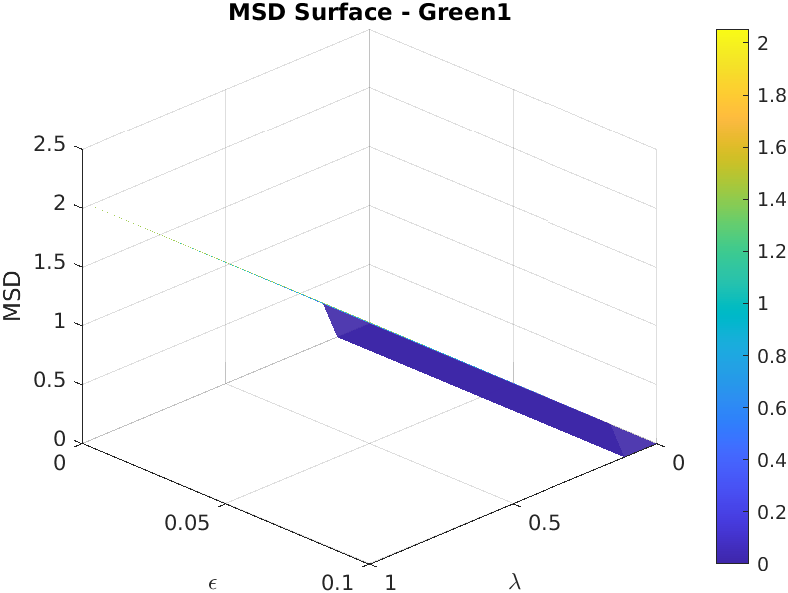
\includegraphics[width=0.7\textwidth]{../utils/results/msd_surfaces/msd_surface_green1_angle_135_30.png}
\caption{Green1 Plane – MSD surface, view angle $(135^\circ, 30^\circ)$}
\end{figure}
\clearpage

\begin{figure}[h!]
\centering
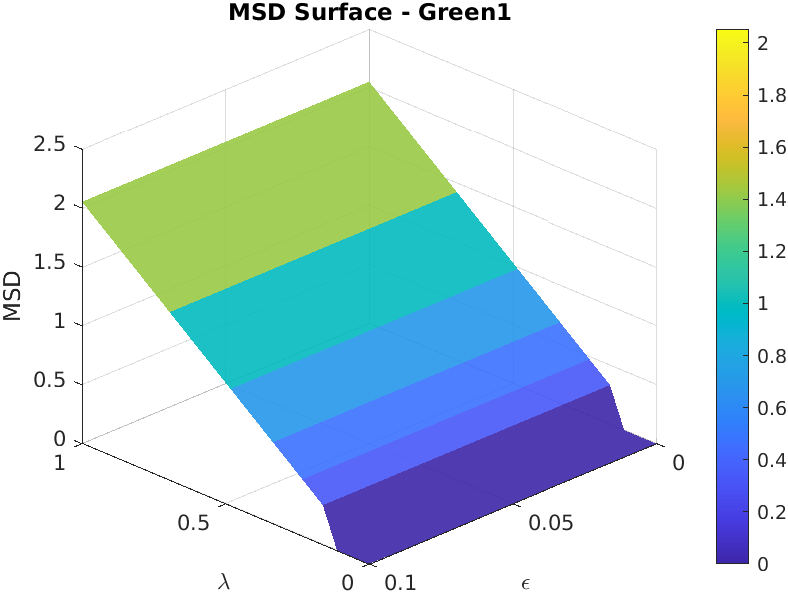
\includegraphics[width=0.7\textwidth]{../utils/results/msd_surfaces/msd_surface_green1_angle_225_30.png}
\caption{Green1 Plane – MSD surface, view angle $(225^\circ, 30^\circ)$}
\end{figure}
\clearpage

\subsection*{Green2 Plane}
\begin{figure}[h!]
\centering
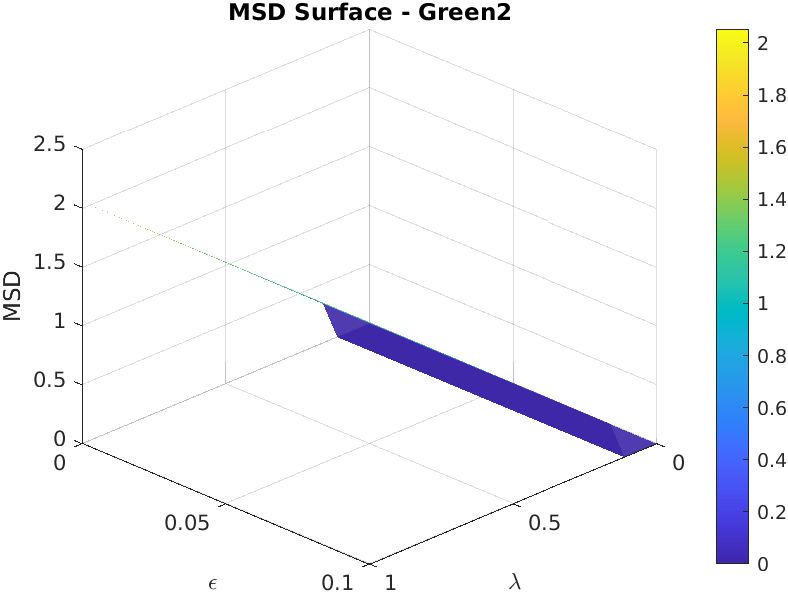
\includegraphics[width=0.7\textwidth]{../utils/results/msd_surfaces/msd_surface_green2_angle_135_30.png}
\caption{Green2 Plane – MSD surface, view angle $(135^\circ, 30^\circ)$}
\end{figure}
\clearpage

\begin{figure}[h!]
\centering
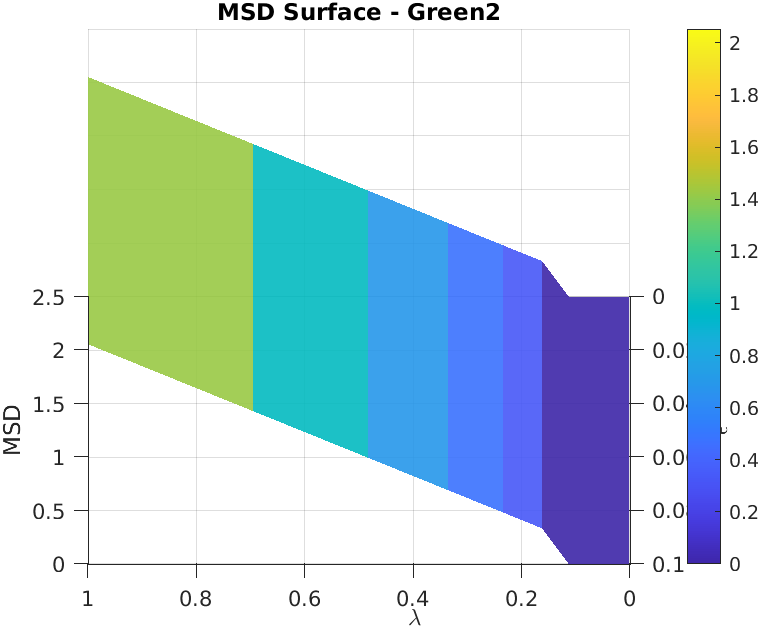
\includegraphics[width=0.7\textwidth]{../utils/results/msd_surfaces/msd_surface_green2_angle_180_45.png}
\caption{Green2 Plane – MSD surface, view angle $(180^\circ, 45^\circ)$}
\end{figure}
\clearpage

\subsection*{Blue Plane}
\begin{figure}[h!]
\centering
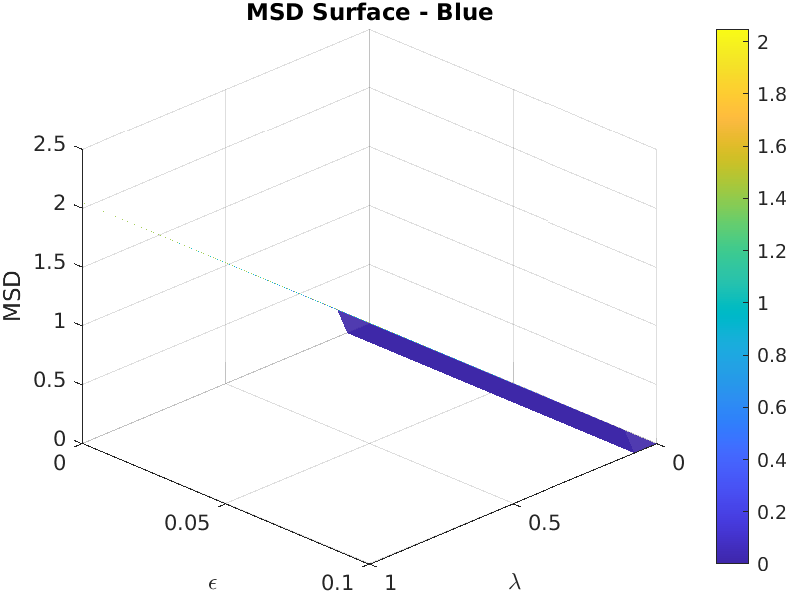
\includegraphics[width=0.7\textwidth]{../utils/results/msd_surfaces/msd_surface_blue_angle_135_30.png}
\caption{Blue Plane – MSD surface, view angle $(135^\circ, 30^\circ)$}
\end{figure}
\clearpage

\begin{figure}[h!]
\centering
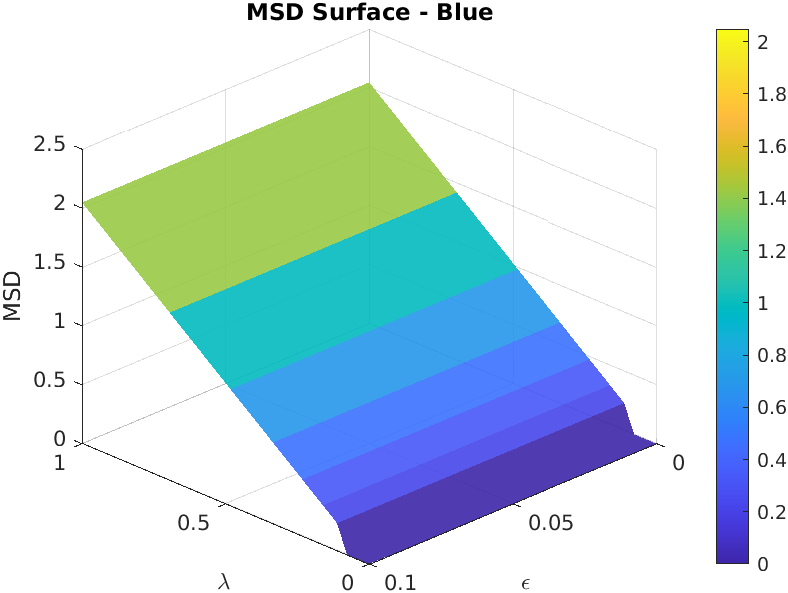
\includegraphics[width=0.7\textwidth]{../utils/results/msd_surfaces/msd_surface_blue_angle_225_30.png}
\caption{Blue Plane – MSD surface, view angle $(225^\circ, 30^\circ)$}
\end{figure}
\clearpage

\noindent These views reinforce the conclusion that:
\begin{itemize}
  \item \textbf{Green planes} exhibit a wider range of stable minima, implying more consistent denoising behavior.
  \item \textbf{Red and blue} surfaces have steeper valleys, reflecting higher noise sensitivity to $(\lambda, \epsilon)$ choices.
  \item The multi-angle views help confirm the global trends in MSD across channels and explain the need for green channel oversampling.
\end{itemize}
\clearpage

\section*{Discussion}
The ROF model demonstrates strong noise suppression while preserving edges. We observed that:
\begin{itemize}
  \item Increasing \(\lambda\) increases smoothing — reduces MSD but can oversmooth.
  \item Smaller \(\epsilon\) preserves edges better but is more sensitive to noise.
  \item A mid-range \((\lambda, \epsilon)\) provides a good trade-off.
\end{itemize}

\subsection*{Bayer Design Insight}
Two green pixels per 2×2 block boost horizontal and vertical luminance sampling — helping demosaicing and noise rejection in green-dominant vision. Our MSD trends empirically support this hypothesis.

\section*{Validation and Testing}
We built a robust test suite with over a dozen tests:

\subsection*{Automated Tests}
\begin{itemize}
  \item \textbf{Zero noise recovery:} flat input returns MSD = 0.
  \item \textbf{Monotonicity:} MSD increases with \(\lambda\).
  \item \textbf{Boundary conditions:} edge gradients remain zero.
  \item \textbf{GPU fallback:} system detects GPU and falls back to CPU if needed.
  \item \textbf{Output shape and batching:} 4D arrays handled correctly.
  \item \textbf{Numerical stability:} solver produces no NaNs/Infs.
  \item \textbf{CPU vs GPU equivalence:} relative error within tolerance (≈3.87\%).
\end{itemize}

\subsection*{Visual Tests}
We used side-by-side comparisons of denoised images and difference maps:

\begin{figure}[h]
    \centering
    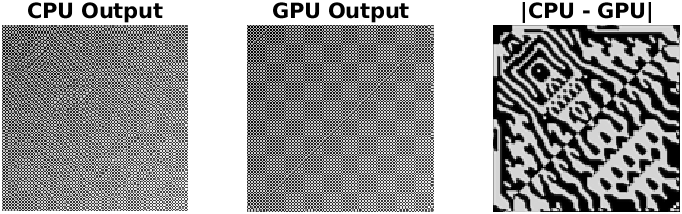
\includegraphics[width=\textwidth]{test/plots/cpu_gpu_diff.png}
    \caption{CPU vs GPU output: Left: CPU, Center: GPU, Right: Difference (amplified).}
\end{figure}

\section*{Performance Benchmarks}
\begin{itemize}
  \item CPU (4 threads): 32 seconds for full grid
  \item GPU (NVIDIA): 2.8 seconds per sweep
  \item Hybrid CPU+GPU (parfor): 9 seconds total
\end{itemize}

\section*{Conclusion}
This project demonstrates the power of variational image processing. The ROF model yields interpretable, tunable results and adapts well to modern hardware. From raw sensor data to smoothed results, we explored denoising quantitatively and visually — revealing both engineering and perceptual truths in digital imaging.

\appendix
\section*{Code Files}
\begin{itemize}
  \item \texttt{smooth\_image\_rof.m} – Main solver with CPU/GPU support
  \item \texttt{calculate\_msd.m} – Computes MSD for parameter grid
  \item \texttt{cpu\_plane\_sweep.m}, \texttt{gpu\_plane\_sweep.m} – Adaptive batching
  \item \texttt{smart\_grid\_search.m} – Coarse-to-fine MSD grid optimization
  \item \texttt{foreach\_plane\_search.m} – Runs search on R/G1/G2/B
  \item \texttt{run\_rof\_hpc.m} – Parallel execution script
  \item \texttt{test/run\_all\_tests.m} – Runs full suite with logging
\end{itemize}

\section*{References}
\begin{itemize}
  \item Rudin, Osher, Fatemi. “Nonlinear total variation based noise removal algorithms.” Physica D, 1992.
  \item Bayer, B.E. “Color Imaging Array.” Eastman Kodak Co., US Patent 3,971,065 (1976).
\end{itemize}

\end{document}

% End of file

